%%%%%%%%%%%%%%%%%%%%%%%%%%%%%%%%%%%%%%%%%%%%%%%%%%%%%%%%%%%%%%%%%%%%%%%%%%%%%%%%%%%
%%%%%%%%%%%%%%%%%%%%%%%%%%%%%%%%%%%%%%%%%%%%%%%%%%%%%%%%%%%%%%%%%%%%%%%%%%%%%%%%%%%
%                               START KAPITEL 1 
%%%%%%%%%%%%%%%%%%%%%%%%%%%%%%%%%%%%%%%%%%%%%%%%%%%%%%%%%%%%%%%%%%%%%%%%%%%%%%%%%%%
%%%%%%%%%%%%%%%%%%%%%%%%%%%%%%%%%%%%%%%%%%%%%%%%%%%%%%%%%%%%%%%%%%%%%%%%%%%%%%%%%%%

\section[Einführung]{Einführung in Schaltvorgänge}
\label{sec:einfuehrung}
\begin{frame}\ftx{\secname}
\s{%
	% Einführung 
	Schaltvorgänge sind Ausgleichsvorgänge, welche unmittelbar nach dem Schalten in elektrischen Netzwerken auftreten.
	Wie der Begriff \glqq elektrische Schaltung\grqq\ im Deutschen vermuten lässt, spielt das Schalten eine große Rolle in der Elektrotechnik. 
	Selbst elektrische Netzwerke, in denen nicht geschalten wird, werden gemeinhin als Schaltungen bezeichnet.

	% Beispiele
	Schalter finden vielfältig Anwendung unter anderem in der Leistungselektronik, der Informations-, der Kommunikations- 
	und der Regelungstechnik. Dabei kommt es nach jedem effektiven Schalten zu Ausgleichsvorgängen, 
	die mitunter erwünschte oder unerwünschte Effekte hervorrufen können.

	% Themen Eingrenzung
	In diesem Modul liegt der Fokus auf der Untersuchung dieser Ausgleichsvorgänge.
}
\begin{Lernziele}{Einführung}
	Studierende lernen: 
	\begin{itemize}
		\item Schaltvorgänge als nicht-stationäre Zustände nach Schaltaktionen kennen % Wissen
		\item Schaltvorgänge im Kontext anderer Ausgleichsvorgänge zu verstehen % Verstehen
		\item Herausforderungen und Möglichkeiten bei Schaltvorgängen kennen % Wissen, Anwenden (Beispiele Praxis, LE, Filter, Verzögerungen, ...)
		\item das Schaltverhalten von idealen und realen Schaltern zu unterscheiden % Verstehen
	\end{itemize}
\end{Lernziele}
\end{frame}



%%%%%%%%%%%%%%%%%%%%%%%%%%%%%%%%%%%%%%%%%%%%%%%%%%%%%%%%%%%%%%%%%%%%%%%%%%%%%%%%%%%%%%%%%%%%%%%%%%

\subsection{Ausgleichsvorgänge}
\label{sec:einfuehrung:ausgleichsvorgaenge}
\begin{frame}\ftx{\subsecname}
\s{%
	% Vorstellung: Ausgleichsvorgänge
	Ausgleichsvorgänge sind allgemein Vorgänge, in denen ein System nach einer Störung einem Gleichgewichtszustand zustrebt.
	
	% Analogien
	Ein Blick in die Physik zeigt, dass Ausgleichsvorgänge auf mannigfaltige Art und Weise in vielen Bereichen vorkommen. 
	Nach dem zweiten Hauptsatz der Thermodynamik strebt ein System stets einem Gleichgewichtszustand zu.
	Demnach kann jeder Vorgang bei entsprechenden Systemgrenzen als Ausgleichsvorgang betrachtet werden.
	Ein Stückweit lassen sich Schaltvorgänge mittels Analogien zu anderen Ausgleichsvorgängen beschreiben.  
	% Alle Vorgänge? 2. Satz Thermodynamik -> Makroskopisch? ... Mh...
	
	% Beispiele
	Beispiele für Ausgleichsvorgänge sind das Erhitzen einer Flüssigkeit, das Ausschwingen eines Pendels oder der Regelvorgang eines Regelkreises.

	\begin{figure}[H]\centering
		% Bild: Bartolomeo Pinelli, Ausschnitt aus \textit{A Peasant Family Cooking over a Campfire}, CC0 1.0. \url{https://commons.wikimedia.org/w/index.php?curid=81414513}
		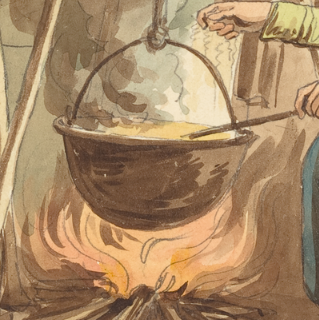
\includegraphics[width=0.3\textwidth]{Bilder/Ausschnitt_A_Peasant_Family_Cooking_over_a_Campfire_by_Bartolomeo_Pinelli_CC0_1.0.png} % 320x319px
		\caption{Erhitzen einer Flüssigkeit\protect\footnotemark}\label{fig:einfuehrung:ausgleichsvorgang:temperaturausgleich}
	\end{figure}
	\footnotetext{Bartolomeo Pinelli, Ausschnitt aus \textit{A Peasant Family Cooking over a Campfire}, Lizenz CC0 1.0\newline\qquad\url{https://commons.wikimedia.org/w/index.php?curid=81414513}}
		
	%Beispiel aperiodisch (DGL 1. Ordnung):\\
	%	Temperaturausgleich. Warum? Energieniveaus anschaulich und Irreversibilität (Entropiesteigerung) (klassisch)

	%Beispiel periodisch (DGL 2. Ordnung):\\
	%	Federpendel. Passt zu \glqq Einschwingvorgängen\grqq. (klassisch)

	%Beispiel periodisch (DGL 2. Ordnung):\\ 
	%	Vergleich Regelung (Motorik). Passt, weil rechnerisch gleich und abgedeckt in Definition ($\rightarrow$ stationärer Zustand)
	%	(Praktisch wegen Überschwingen)
}%
\b{%
	\begin{minipage}{\textwidth}% Obere Hälfte
		\begin{minipage}{0.48\textwidth}\centering
			\resizebox{0.9\textwidth}{!}{\includegraphics{Tikz/pdf/circ_switchable_rc_charge_dc.pdf}}
		\end{minipage}%
		\begin{minipage}{0.48\textwidth}\centering
			\includegraphics{Tikz/pdf/plot_rc_charge_uc_transition.pdf}
		\end{minipage}
	\end{minipage}
	\vspace{0.5cm}
	\pause

	\begin{minipage}{\textwidth}% Untere Hälfte
		\begin{minipage}[t]{0.48\textwidth}\centering
			\underline{Analogie: Wasser erhitzen}\footnotemark
			\vspace{2mm}

			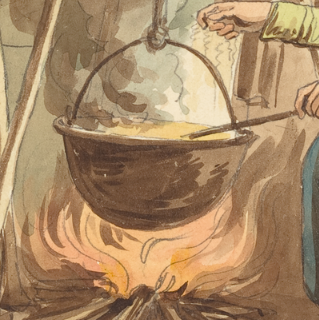
\includegraphics[width=0.4\textwidth]{Bilder/Ausschnitt_A_Peasant_Family_Cooking_over_a_Campfire_by_Bartolomeo_Pinelli_CC0_1.0.png}%
			\pause
		\end{minipage}%
		\begin{minipage}[t]{0.48\textwidth}%\centering
			\underline{Ursachen für Ausgleichsvorgänge:}
			\vspace{2mm}
			\begin{itemize}
				\item Schalthandlungen
				\item DC: Änderung d. Spannung/Strom
				\item AC: Änderung d. Frequenz/Amplitude/Phase
			\end{itemize}
		\end{minipage}
	\end{minipage}
	\footnotetext{Bild: Bartolomeo Pinelli, Ausschnitt aus \textit{A Peasant Family Cooking over a Campfire}, Lizenz CC0 1.0\newline\qquad\url{https://commons.wikimedia.org/w/index.php?curid=81414513}}
}
\end{frame}

\b{% Beamer only, extra frame
\begin{frame}\ftx{\subsecname\,- Beispiele}
	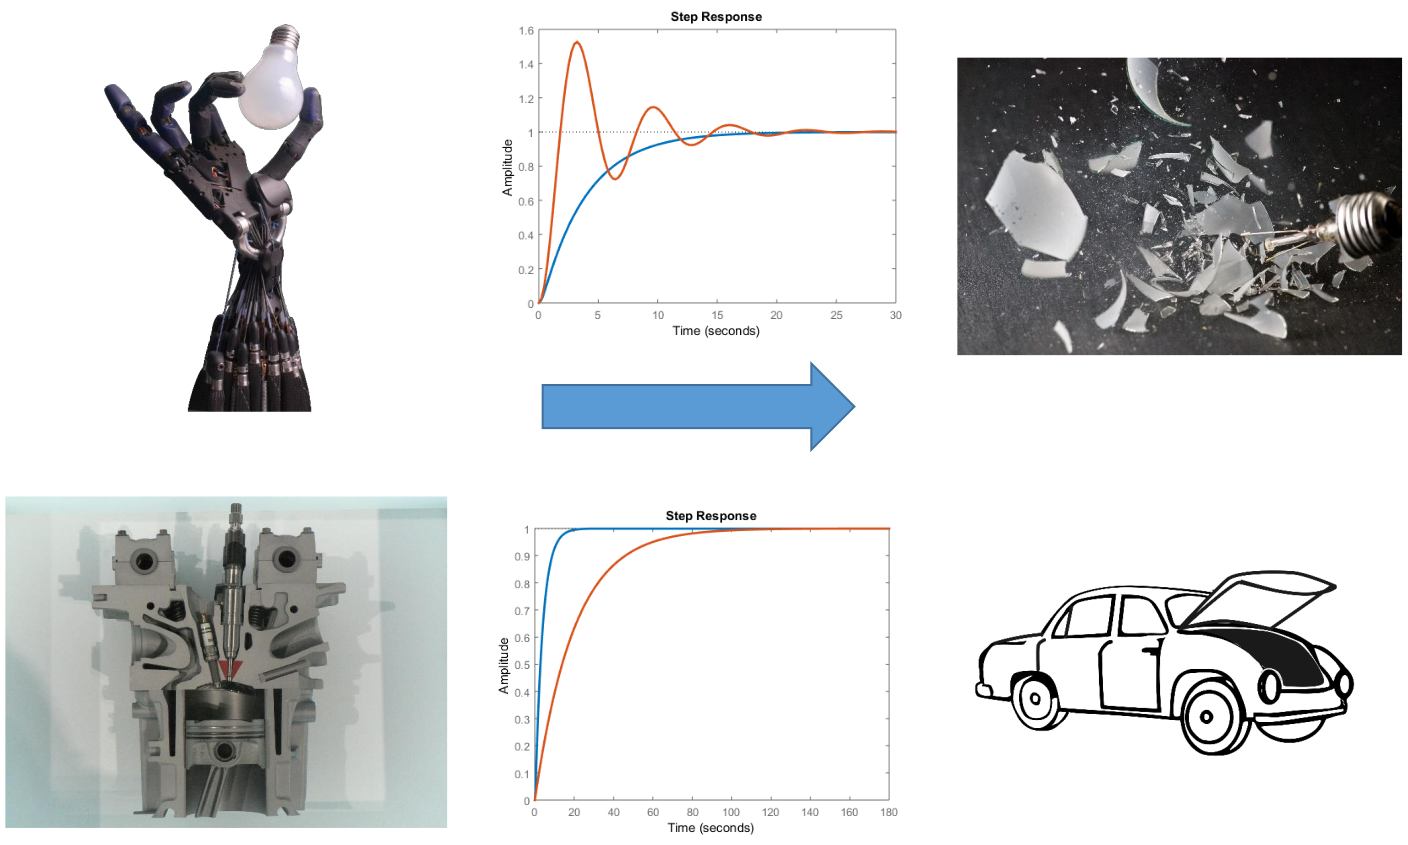
\includegraphics[width=\textwidth]{Bilder/Ausgleichsvorgaenge_Beispiele_ET3_S_Exknowski_FH_SWF.png}% Provisorisch mit Genehmigung von Prof. Exknowski
\end{frame}
}
%%%%%%%%%%%%%%%%%%%%%%%%%%%%%%%%%%%%%%%%%%%%%%%%%%%%%%%%%%%%%%%%%%%%%%%%%%%%%%%%%%%%%%%%%%%%%%%%%%

\subsection{Schaltvorgänge}
\label{sec:einfuehrung:schaltvorgaenge}
\begin{frame}\ftx{\subsecname}
\s{
	% Def: Schaltvorgang, Prämisse (idealer Schalter)
	Als Schaltvorgänge werden Ausgleichsvorgänge unmittelbar \underline{nach} dem Schalten bezeichnet.
	Diese sind Hauptgegenstand des Moduls, wobei hierfür stehts von idealen Schaltern ausgegangen wird.

	% Bild: Schaltvorgang DC, AC
	Abbildung \ref{fig:plot:transient_persistent} zeigt exemplarisch den Zeitverlauf einer 
	Systemgröße $s(t)$ (z.B. Strom oder Spannung) während eines Schaltvorgangs. 
	Zum Vergleich sind für das Zuschalten einer Anregung zwei Fälle dargestellt:
	einmal für eine Gleichgröße (DC) und einmal für eine Wechselgröße (AC).
}
% Bsp. Einschwingvorgang nach Schalten als Schaltvorgang. Vgl. DC und AC 
\b{\centering Beispiel Schaltvorgang bei Gleich- und Wechselspannung.
}%
\fu{\includegraphics{Tikz/pdf/plot_transient_persistent.pdf}}%
	{Vergleich: Ausgleichsvorgang AC, DC\label{fig:plot:transient_persistent}}
\s{
	% Bild-Erklärung: Vorgänge, Zustände
	% stationär -> Schalten (instantan) -> Schaltvorgang (transient) -> stationärer Zustand (persistent)
	Der dargestellte Schaltvorgang beginnt mit dem Schalten bei $t=0$ (gestrichelte Grenze, links) 
	und endet mit Erreichen eines stationären Zustands (persistent) (gestrichelte Grenze, mittig).
	Der stationäre Zustand von $s(t)$ entspricht
	bei Anregung mit Gleichgröße (DC) ebenfalls einer Gleichgröße (konstant) und
	bei Anregung mit Wechselgröße (AC) ebenfalls einer Wechselgröße (periodisch). 

	Der in Abb. \ref{fig:plot:transient_persistent} dargestellte Vorgang beim Übergang (transient) 
	von Schalten bis Erreichen eines stationären Zustands kann hier auch als 
	Ausgleichsvorgang (allgemein), Schaltvorgang (speziell) oder Einschwingvorgang (speziell) bezeichnet werden. 

	% Abgrenzung: Vorgänge beim Schalten (realer Schalter)
	Ausgleichsvorgänge \underline{während} dem Schalten, wie sie bei realen Schaltern auftreten,
	werden nicht als Schaltvorgänge bezeichnet und in diesem Modul nicht näher untersucht. 
	Eine kurze Erläuterung findet sich jedoch vollständigkeitshalber in Abschnitt \ref{sec:einfuehrung:schalteridealvsreal} 
	beim Vergleich idealer und realer Schalter.
}
\end{frame}

%%%%%%%%%%%%%%%%%%%%%%%%%%%%%%%%%%%%%%%%%%%%%%%%%%%%%%%%%%%%%%%%%%%%%%%%%%%%%%%%%%%%%%%%%%%%%%%%%%

\subsection{Beispiele für Schaltvorgänge}
\label{sec:einfuehrung:beispieleschaltvorgaenge}
\begin{frame}\ftx{\subsecname}
% Anwendungsbereiche von Schaltungstechnik: Leistungselektronik, Kommunikationstechnik(?), ...
\b{% Beamer only
\textbf{Beispiel aus der Leistungselektronik:} 

\begin{minipage}{0.38\textwidth}\centering
	\includegraphics[width=\textwidth]{Bilder/Tiefsetzsteller_Schaltung_GET2_J_Böcker_Uni_Paderborn_cut.png}
	Tiefsetzsteller mit Glättungskondensator\footnotemark
\end{minipage}%
\begin{minipage}{0.58\textwidth}\centering
	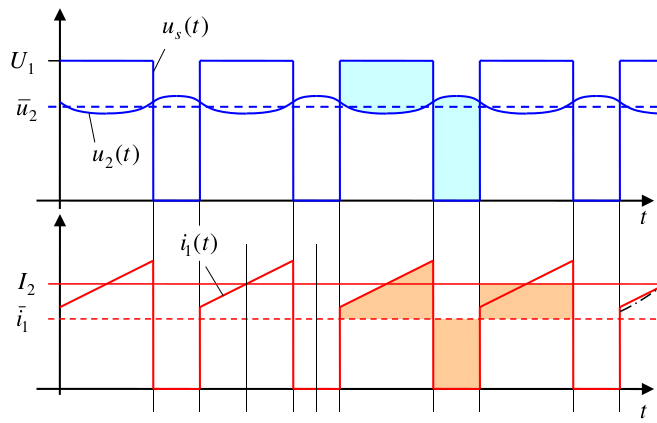
\includegraphics[width=0.9\textwidth]{Bilder/Tiefsetzsteller_Zeitverläufe_GET2_J_Böcker_Uni_Paderborn_cut_edit.png}
\end{minipage}
\footnotetext{Schaltbild und Zeitverlauf: Joachim Böcker, GET2, Universität Paderborn, modifiziert (gekürzt)}

Stromrichter (engl. \textit{power converter}) wandeln elektrische in elektrische Energie um 
Die Wandlung (z.B. Spannung, Strom, Frequenz) erfolgt durch getaktetes Schalten.\vspace{5pt}

\textbf{Andere Beispiele:}\\
Ein-/Ausschalten, AD-/DA-Converter, Fahrradlicht mit Kondensator, ...
}% end Beamer only
\s{% Skript only
	Prinzipiell kommt es bei jedem Schalten in elektrischen Netzwerken zu Schaltvorgängen. 
	
	Typische Beispiele sind Umrichter (engl. \textit{power converter}) in der Leistungselektronik,
	welche elektrische Energie in eine andere Form elektrischer Energie umwandeln. 
	Durch gezieltes Schalten von Halbleiterbauelementen (z.B. Transistoren, Thyristoren) 
	kann die Spannung, der Strom oder die Frequenz verändert werden. 
	In jedem Taktzyklus werden Kapazitäten und Indukivitäten abwechselnd geladen und entladen. 
	
	Abbildung \ref{fig:circ:pulldown} zeigt beispielhaft eine Tiefsetzsteller (Buck-Converter) mit Glättungskondensator.
	Dieser wandelt eine Gleichspannung $U_1$ in eine niedrigere Gleichspannung $U_2$ um. 
	Daneben sind in Abbildung \ref{fig:plot:pulldown} die zeitlichen Verläufe von Spannungen und Strömen
	jeweils am Eingang und am Ausgang des Tiefsetzstellers dargestellt.

	\begin{figure}[H]\centering
		\begin{subfigure}{0.5\textwidth}\centering
			\includegraphics[width=\textwidth]{Bilder/Tiefsetzsteller_Schaltung_GET2_J_Böcker_Uni_Paderborn_cut.png}
			\caption{Schaltbild eines Tiefsetzstellers (Buck-Converter)}
			\label{fig:circ:pulldown}
		\end{subfigure}%
		\begin{subfigure}{0.5\textwidth}\centering
			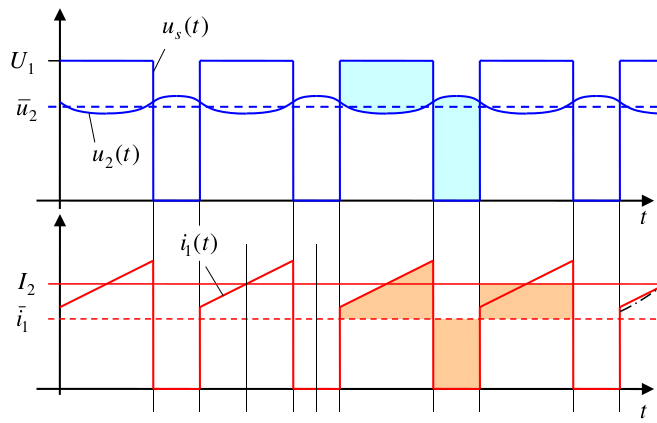
\includegraphics[width=0.9\textwidth]{Bilder/Tiefsetzsteller_Zeitverläufe_GET2_J_Böcker_Uni_Paderborn_cut_edit.png}
			\caption{Zeitverlauf von $u(t)$ und $i(t)$ am Tiefsetzsteller}
			\label{fig:plot:pulldown}
		\end{subfigure}
		\caption{Beispiel: Schaltvorgänge am Tiefsetzsteller\protect\footnotemark}
	\end{figure}
	\footnotetext{Quelle: Schaltbild und Zeitverlauf (modifiziert, gekürzt): Joachim Böcker, GET2, Universität Paderborn}

	Ohne nähere Rechnung ist erkennbar, dass die Ausgangsspannung auch im stationären Betrieb nicht konstant ist.
	Die Ausgangsspannung über dem Glättungskondensator schwankt, da sich die Kapazität in jeder Schaltperiode 
	etwas entlädt und wieder auflädt. 
	
	Mithilfe der Methoden aus diesem Modul lassen sich solche Schaltvorgänge berechnen und analysieren. 
	Zum besseren Verständnis werden in Kapitel \ref{sec:schaltvorgaengezeitbereich} jedoch einfachere Beispiele von
	Schaltvorgänge ohne periodisches Schalten betrachtet.

	Andere Beispiele für Schaltvorgänge sind das Ein- und Ausschalten von Geräten,
	Analog-Digital- und Digital-Analog-Wandlung, das Aufladen eines Kondensators durch ein Fahrradlicht.
}

	%Bei elektrischen Schaltvorgängen: Schalter (Ein/Aus), Relais, Transistoren, ...
%
	%Leistungselektronik überwiegend Schaltungselektronik im wortwörtlichen Sinne. 
	%%( DC <---DC/AC ---> AC)
	%%( î  .           .  î )
	%%( |    .       .    | )
	%%( |      .   .      | )
	%%(DC/DC     X     AC/AC)
	%%( |    .       .    | )
	%%( v  .           .  v )
	%%( DC <---DC/AC ---> AC)
%
	%DC/AC: Wechselrichter (U,f,phi)\\
	%AC/AC: Frequenzumrichter (f) / Phasenregler (phi) / AC-Spannungsregler (U,(f),(phi))\\
	%DC/DC: Hochsetz-/Tiefsetz-/Hochtiefsetz-steller / DC-Spannungsregler (U)\\
	%AC/DC: Gleichrichter (U)\\

\end{frame}

%%%%%%%%%%%%%%%%%%%%%%%%%%%%%%%%%%%%%%%%%%%%%%%%%%%%%%%%%%%%%%%%%%%%%%%%%%%%%%%%%%%%%%%%%%%%%%%%%%

\subsection{Vergleich idealer und realer Schalter}
\label{sec:einfuehrung:schalteridealvsreal}
\begin{frame}\ftx{\subsecname}
\s{
	% Intro: Reales Schalten
	Zur Vereinfachung wird in diesem Modul stets von idealen Schaltern ausgegangen.
	Um die Grenzen dieser Annahme zu verstehen, wird im Folgenden der Unterschied zwischen idealen und realen Schaltern erläutert.
	Hierfür wird wie im Schaltbild in Abbildung \ref{fig:circ:switch} gezeigt ist, die Schalterspannung über einem Schalter betrachtet.
	Der Schalter ist hierfür an eine lineare Gleichspannungsquelle mit Spannung $U_q$ angeschlossen.
}
\begin{figure}[H]\centering
	\includegraphics{Tikz/pdf/circ_switch_ideal.pdf}
	\s{\caption{Schaltbild, Schalterspannung}}\b{\par Schalterspannung $\ecv{u(t)}$}
	\label{fig:circ:switch}
\end{figure}
\s{
	% Abbildung: Ideal vs. Real
	Abbildung \ref{fig:plot:schalter} zeigt die Schalterspannung im Durchlass- und im Sperrbetrieb und in den Übergangsphasen beim Öffnen oder Schließen des Schalters.
	Links ist der Spannungsverlauf für einen idealen Schalter dargestellt, rechts für einen realen Schalter.
}
\begin{figure}[H]\centering
	\begin{subfigure}{0.48\textwidth}\centering
		\includegraphics{Tikz/pdf/plot_switch_ideal.pdf}
		\s{\caption{Spannung bei idealem Schalter}}\b{\par Ideal: verlustlos, instantan}
		\label{fig:plot:schalter:ideal}
	\end{subfigure}\pause
	\begin{subfigure}{0.48\textwidth}\centering
		\includegraphics{Tikz/pdf/plot_switch_real.pdf}
		\s{\caption{Spannung bei realem Schalter}}\b{\par Real: Verluste, Latenzen}
		\label{fig:plot:schalter:real}
	\end{subfigure}
	\s{\caption{Vergleich: Schaltverläufe bei idealem und realem Schalter}}
	\label{fig:plot:schalter}
\end{figure}
%i(t),u(t)			ideal
%		î
%	U2_	|    ________         ______
%		|   |        |       |
%	U1_	|___|        |_______|
%		|___________________________> t
%
%i(t),u(t)			real
%		î
%	U2_	|..  _______   ....   ______    ___ = Spannung
%		|  ./       \.      ./
%	U1_	|__/ ....... \______/.......    ... = Strom
%		|___________________________> t
\end{frame}
\begin{frame}\ftx{\subsecname}
\s{
	% Beschreibung: Ideal vs. Real
	Ein idealer Schalter wechselt beim Schalten instantan und verlustlos 
	von einem leitenden Zustand ($R=0$) zu einem sperrenden Zustand ($G=0$) oder umgekehrt
	wie in Abbildung \ref{fig:plot:schalter:ideal} dargestellt ist.
	Ein realer Schalter hingegen leitet oder sperrt nicht instantan
	wie in Abb. \ref{fig:plot:schalter:real} vereinfacht dargestellt ist. 
	Stattdessen treten Latenzen und Verluste auf.
	Im Durchlassbetrieb liegt immernoch eine kleine Spannung an (Durchlasswiderstand $R>0$)
	und im Sperrbetrieb fließt immernoch ein kleiner Strom (Sperrleitwert $G>0$).
	Dadurch kommt es zu Verlusten im Schalter, insbesondere während der Übergangsphasen, wenn sowohl Spannung als auch Strom anliegen.
	
	% Erklärung
	Die Latenzen und Verluste realer Schalter resultieren aus deren resistiven, induktiven und kapazitiven Eigenschaften.
	Aufgrund dieser Eigenschaften ist Schalten real betrachtet - schalterintern - immer mit Ausgleichsvorgängen verbunden.
	In der Praxis werden solche Effekte, wenn unerwünscht, als parasitär bezeichnet.
	
	% Beispiel: MOSFET
	Abbildung \ref{fig:circ:mosfet} zeigt exemplarisch einen MOSFET als Schalter zur Veranschaulichung. 
	Zum Vergleich ist der MOSFET einmal ideale (ohne) und einmal real (mit kapazitiven Effekten) dargestellt.
}
% Ref: http://fmh-studios.de/theorie/mosfet/schaltverhalten/
\begin{figure}[H]\centering
	\begin{subfigure}{0.48\textwidth}\centering
		\includegraphics{Tikz/pdf/circ_mosfet_ideal.pdf}
		\s{\caption{MOSFET, ohne Kapazitäten (ideal)}}\b{Ideal: keine parasitären Effekte}
		\label{fig:circ:mosfet:ideal}
	\end{subfigure}%
	\onslide<2->{%
	\begin{subfigure}{0.48\textwidth}\centering
		\includegraphics{Tikz/pdf/circ_mosfet_capacitive_effects.pdf}
		\s{\caption{MOSFET, inkl. Kapazitäten (real)}}\b{Real: mit parasitären Kapazitäten}
		\label{fig:circ:mosfet:kapazitiv}
	\end{subfigure}
	}% end onslide
	\s{\caption{Vergleich: Schaltung mit MOSFET, ohne (ideal) und mit kapazitiver Effekte (real)}}
	\label{fig:circ:mosfet}
\end{figure}
\s{
	%Der MOSFET wird am Drain-Anschluss über einen Widerstand $R$ mit einer konstanten Gleichspannung ($5\ \mathrm{V}$ Potential) versorgt.
	%Das Potential am Source-Anschluss ist auf konstant $0\ \mathrm{V}$ gelegt. 
	%Die Eingangsspannung $\underline{U}_1$ liegt zwischen Gate und Source an,
	%die Ausgangsspannung $\underline{U}_2$ zwischen Drain und Source.

	% Erklärung Latenzen, Abgrenzung
	Die kapazitiven Effekte zwischen den Anschlüssen des MOSFETs führen zu einer Verzögerung beim Schalten,
	da die jeweiligen Kapazitäten während des Schaltens erst geladen beziehungsweise entladen werden müssen.
	Das MOSFET-Beispiel dient lediglich zur Veranschaulichung der Unterschiede zwischen idealen und realen Schaltern.
	Ausgleichsvorgänge während Schaltaktionen werden in diesem Modul nicht weiter betrachtet.
	Mit Schaltvorgängen sind immer die Ausgleichsvorgänge \underline{nach} dem Schalten gemeint.
}%
\b{%
	\makebox[2cm][l]{\textbf{Hier:}} Ausgleichsvorgänge \makebox[1.5cm][c]{\underline{nach}} Schalten (Schaltvorgänge) im Fokus
	%\\\qquad$\rightarrow$ Annahme idealer Schalter %(verlustlos, instantan)
	\\[+4pt]%
	\makebox[2cm][l]{\textbf{Real:}} Ausgleichsvorgänge \makebox[1.5cm][c]{\underline{während}} Schalten
	%\\\qquad$\rightarrow$ Schaltverluste und Latenzen
	\\[+4pt]%
	\makebox[2cm][l]{\textbf{Eingrenz.:}} Annahme idealer Schalter 
}
\end{frame}

%%%%%%%%%%%%%%%%%%%%%%%%%%%%%%%%%%%%%%%%%%%%%%%%%%%%%%%%%%%%%%%%%%%%%%%%%%%%%%%%%%%%%%%%%%%%%%%%%%

%\subsection{...}
%\label{sec:...}
%\begin{frame}\ftx{\subsecname}
%\end{frame}

%-------------------------------------------------------------------------------------------------%
